%\subsection{Latin Hypercube Sampling}\label{sec:LHsamp}
One of the cheapest sampling strategies is stratified sampling.
The easiest variant to describe, viz.\ Latin hypercube~\cite{Mc79Comp}
is illustrated in \Fig{hcube},
after Steinberg as quoted in ref~\cite[\S\,4]{kaloswhitlock}.
The sample space is gridded, but now sample
points are required to lie within the grid squares, and in fact their
precise location within a square in determined randomly.
The selection of grid-square is also random, but heavily constrained
by the fact that no other sampled square should have the same
discrete co-ordinate values in any co-ordinate. For example,
in \Fig{hcube}, the fact that there is a sample point in the
square three along from the left in the bottom row, discrete
coordinate~$(3,1)$, means that no sample will be placed in
cells with coordinates~$(3,j)$ or~$(i,1)$ for any~$i$ or~$j$.
If there are~$N_1$ cells in each coordinate, the
total number of samples needed is also~$N_1$.
This is very cheap, but the method is known to
become unreliable when the parameters' variations are correlated.
\begin{figure}
\centerline{\rotatebox{0}{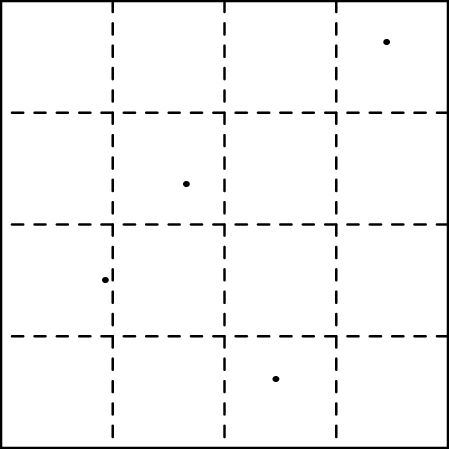
\includegraphics[width=6.5cm]{../png/hcube}}}
\caption{\label{fig:hcube}
 Latin hypercube sampling.}
\end{figure}
